%http://onlinelibrary.wiley.com/doi/10.1002/dvdy.23844/full

\documentclass[12pt]{article}
\usepackage{url}
\usepackage{listings}
\usepackage{graphicx}
\begin{document}

\title{Datatube: a GUI for visualizing differential expression}
\author{Author:
			\\Josefina Correa
			\\josefina.correa@upr.edu
            \\Biology Department
            \\University of Puerto Rico-Rio Piedras
            \\	
            \\Advisor:
            	\\Humberto Ortiz-Zuazaga
                \\humberto@hpcf.upr.edu
                \\Computer Science Department
                \\University of Puerto Rico-Rio Piedras}
            			

\maketitle
\begin{abstract}
Differential expression analysis of genes and/or transcripts is a tool that aids in characterizing a cellular environment under different circumstances. The echinoderm \textit{Holothuria glaberrima} is a non-model organism with the attribute of being able to regenerate nearly any injured part fairly quickly. The Datatube GUI was designed for the purpose of exploring differential expression in contigs obtained by \textit{de novo} assembly of this organism. It contains data for differential expression of contigs of \textit{H. glaberrima's} radial complex. A heatmap is generated from a user-specified subset of these contigs, and can be exported as a .pdf file. The code and documentation is available at \url{http://github.com/josefinacmenendez/Datatube_Heatmap} and the GUI can be accessed at \url{http://josefinacmenendez.shinyapps.io/Datatube_Heatmap}. 

\end{abstract}


\section{Introduction}
\textit{De novo} sequencing is a fundamental research technique that allows for increasing knowledge about several fields that span from evolution and genetics to epidemiology. Increasing knowledge about an organism's genome is important for understanding gene regulation, evolutionary relationships, and even an organism's development. In fact, the more organisms that are sequenced, the greater the knowledge about highly conserved genes. For instance, homologous genes can be used as a proxy for protein-function annotation. \cite{Lowenstein09}  
	
Datatube was generated for the purpose of visualizing data obtained by "deep transcriptome sequencing on mRNA samples from the sea cucumber \textit{H. glaberrima}; these samples were extracted from uninjured and regenerating radial complex at different times: day 2, day 12, and day 20. \cite{Mashanov12} Visualizing the data through heatmaps allows for identifying potential regions of interest and perform further analyses. 

\section{Methods}
To build Datatube, Shiny was used, while shinyapps.io enabled deployment and hosting. Both tools are open source and were developed by RStudio. \cite{shinyapps,shiny,R} Building an app using Shiny requires having two portions of scripts: ui.R (which controls the user interface and layout), and server.R (which compiles the app). An additional portion, global.R, can be included. This segment contains global variables and function definitions. The following scripts were written to design the GUI and were documented on the aforementioned GitHub repository:

\begin{lstlisting}[language=R]
#ui.R
shinyUI(
  
  fluidPage(
  titlePanel("Select Contigs"),
  sidebarLayout(
      sidebarPanel(
      	selectizeInput("contigs", "Select up to 50 contigs", 
                     choices = NULL, 
                     options=list(maxOptions = 100),
                     multiple = TRUE),
      	downloadButton(outputId = "dld", label = "Export as pdf")
                 ),              
    mainPanel(
      plotOutput("histogram")
      )
    )
  )
)

#server.R

shinyServer(function(input,output,session){
 
  updateSelectizeInput(session, 'contigs',	 
  choices = contigs,	 
  server = TRUE,	 
  options = list(maxItems=50))	
  
  output$histogram <- renderPlot({
    validate(need(length(input$contigs)>1,	
    message = "Select at least 2 contigs and 50 contigs at most")) 
    plotHist(input$contigs)
  }, height = 700, width = 1000)

  output$dld <- downloadHandler(
    filename = function(){
      paste("heatmap", "pdf", sep = ".")
    },
    content = function(file) {
      pdf(file, height = 7, width = 10)
      plotHist(input$contigs)
      dev.off()
    }
  )
})


#global.R

library(shiny)
library(gplots)
library(functional)

nvs2 <- read.csv("N_vs_day2_whole_list.csv")
nvs12<- read.csv("N_vs_day12_whole_list.csv")
nvs20<- read.csv("N_vs_day20_whole_list.csv")

contig.number <- nvs2$id

nvs2.log2Foldchange <- nvs2$log2FoldChange
nvs12.log2Foldchange<- nvs12$log2FoldChange
nvs20.log2Foldchange<- nvs20$log2FoldChange

dge_pepino <- cbind(nvs2.log2Foldchange,	
			nvs12.log2Foldchange,	
			nvs20.log2Foldchange)	
colnames(dge_pepino) <- c("Day2","Day12","Day20")
rownames(dge_pepino) <- contig.number

#Remove non-numeric values
dge_pepino <- dge_pepino[apply(dge_pepino, 1, 
				Compose(is.finite, all)), 
				, drop=FALSE]

contigs <- row.names(dge_pepino)
contigs <- as.vector(contigs)

plotHist <- function(conts){
  heatmap.2(dge_pepino[c(conts),], trace = "none", col = redblue(20),
            cexCol = 2,
            cexRow = 0.2 + 1/log10(length(conts)),
            margins = c(8,20))
}
\end{lstlisting}	
\section{Results}	
  \begin{minipage}[b]{\textwidth}
      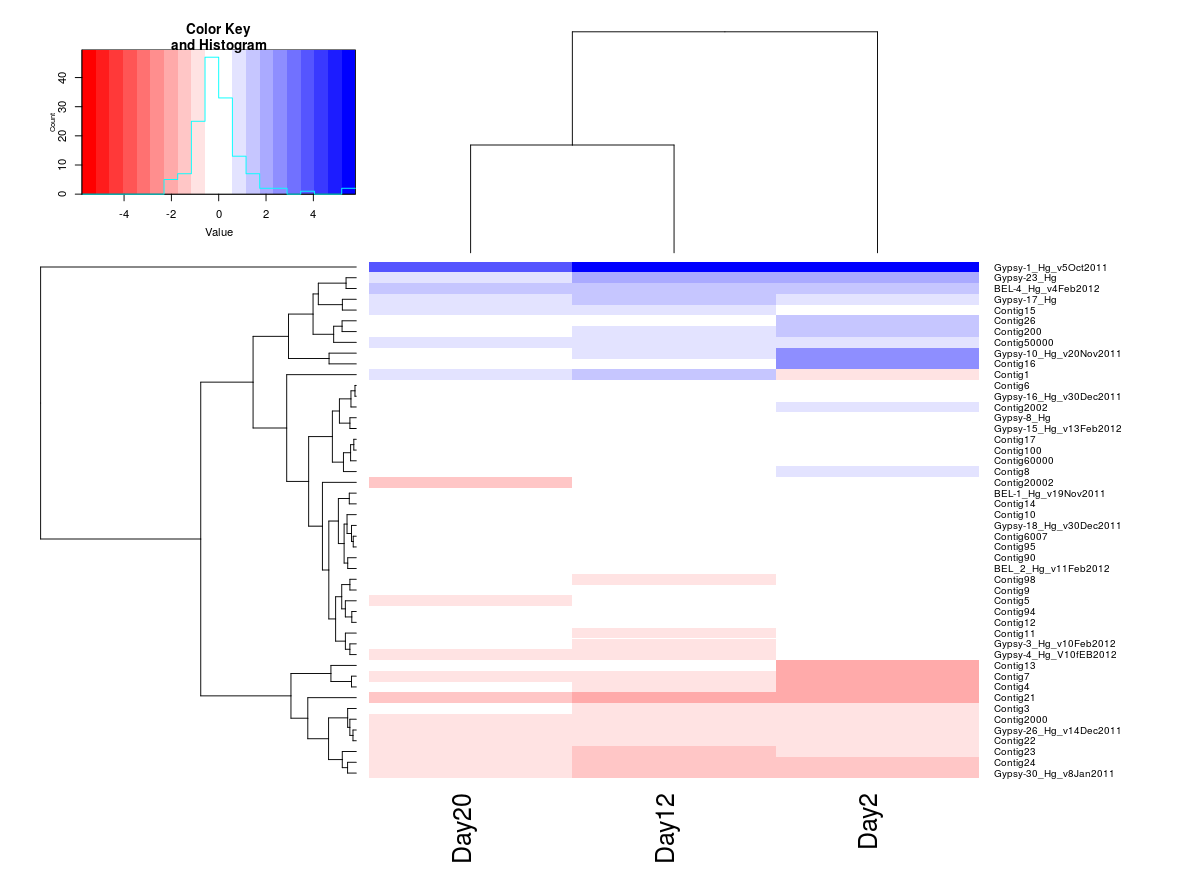
\includegraphics[width=\textwidth]{histogram}
      \textbf{Figure 1: Heatmap showing differential expression for radial 					nerve tissue from \textit{H. glaberrima} at different days.}
  \end{minipage} 
\section{Conclusions}
The GUI is working properly and serves its purpose. However, some aspects should be improved, such as the ease of access to differentially expressed contigs. This, and other details that can be improved, are discussed in the following section.

\section{Future work}
After assembly, the next step is identifying genes or sequences of interest within the contigs, for which BLAST is used. Rather than copying and pasting the contigs, it would be more convenient to access BLAST programmatically and to provide a tool within this GUI to facilitate the process. With this in mind, the following features will be added to the GUI: 

\begin{itemize}
  \item upload data and generating the heatmaps from this data	
  \item filter the data for up-regulated and down-regulated contigs	
  \item export a user-specified subset of contigs	
  \item perform BLAST on the selected contigs	
\end{itemize}


\section{Acknowledgements}
I would like to thank Dr. Humberto Ortiz-Zuazaga for his mentorship and guidance, and my colleagues at the Megaprobe Lab. This project was funded by the IDI-BD2K program grant R25 MD010399. 

\nocite{*}
\bibliographystyle{IEEEannot}
\bibliography{annot}

\end{document}